\section{Tuesday, January 17th: Welcome to User Interface Design and Development}
\subsection{The dangers of poor UI/UX}
It is a nice sunny day, you are relaxing on your vacation in Hawaii. Suddenly, you get an alert on your phone that a missile attack is incoming: and mass panic ensues.

But then it is clarified that there was actually no threat and the message was sent in mistake.

How did this happen?

To answer that question, let us look at the UI: We have a dropdown menu with ambiguous acronyms and a confirmation that follows. However the confirmation that follows highlights the ``Yes'' option as if it is the default.

\subsection{Where did we start}
\subsubsection{The Commandline}
In the Command-line, we had a terminal. Now we have a desktop with icons! Modern UI is organized like a physical office: there's a file cabinet with files and a wastebasket.

\begin{important}
But we should not take the metaphor too far:

Making a 3D VR-ish desktop office on your computer has benefits and downfalls. One major downfall is: you are trying to represent 3D via a 2D screen.
\end{important}

\subsection{Course Staff and Communication}
Here is the CS 160 course staff for this semester!

Bjoern Hartmann: Instructor

Shm Almeda: TA

Peitong Duan: TA

Ace Chen: Reader

Hridhay Suresh: Reader

\subsection{Enrollment}
This class is oversubscribed with $\sim$100 seats total, split between CS 160 (undergrad) and CS 260A (graduate).

We usually see 5-10\% turnover, so if you're in the first 10 positions then you should keep up with the class. Otherwise the chance that you can take the class this semester is unlikely.

Luckily, you can take this class in the summer semester!

Alternatively:
\begin{itemize}
    \item DES INV 15: Design Methoology
    \item DES INV 25: UX Design (non-technical)
    \item IEOR 170: Human Factors
    \item INFO 213: UI Design and Development
    \item INFO 114/214: UX Research
\end{itemize}
are classes you can look into.

\begin{important}
This class has a heavy workload. If you are an EE/CS Major, you already know what upper-division CS classes are like. If you do not think you can handle it, you should drop ASAP to give others a fair chance to get in.

If you are beyond spot 10 on the waitlist, consider leaving now. Likewise if you do not have a seat/cannot see the screen.
\end{important}

\subsection{This Course}
is about reliably building very good interactive systems.

We focus on \textbf{interactions with and 
through intelligent systems.}

The goal of this class is to build a working \textbf{interactive 
prototype.} We do \textit{not} focus on scaling the class to millions of people, for that CS 169 will moreson help you with that -- CS 160 is more for the front-end.

We place emphasis on de-risking via \textbf{user testing} and working on rapidly prototyping.

\subsection{Human-Computer Interaction (HCI)}
Design, prototyping \& evaluation of UIs.

Human
\begin{itemize}
    \item End-user of program
    \item Others (friends, collaborators, coworkers)
\end{itemize}

Computer
\begin{itemize}
    \item The machine the program runs on
    \item Can be (and often is) split: clients \& servers
\end{itemize}

Interaction
\begin{itemize}
    \item User tells the computer what they want
    \item Computer communicates results
\end{itemize}

\subsection{User Interfaces (UI)}
What allows people to interact with computers \& the computer to communicate results.

Note that this can include hardware design (i.e. buttons).

\subsubsection{Why Study User Interfaces?}
\begin{itemize}
    \item In today's applications, an average of 48\% of the code is devoted to the user interface portion -- It's a major part of work for ``real'' programs (approx 50\%).
    \item You work on real software intended for others
    \item Bad UI costs money, lives (see Airplane crash into a canyon due to badly designed UI in autocomplete software that the pilot used), votes, etc
    \item UI is hard to get right -- people are unpredictable.
\end{itemize}

\subsection{Interface Design Cycle}
If you take away anything from this lecture, remember this:
\begin{center}
    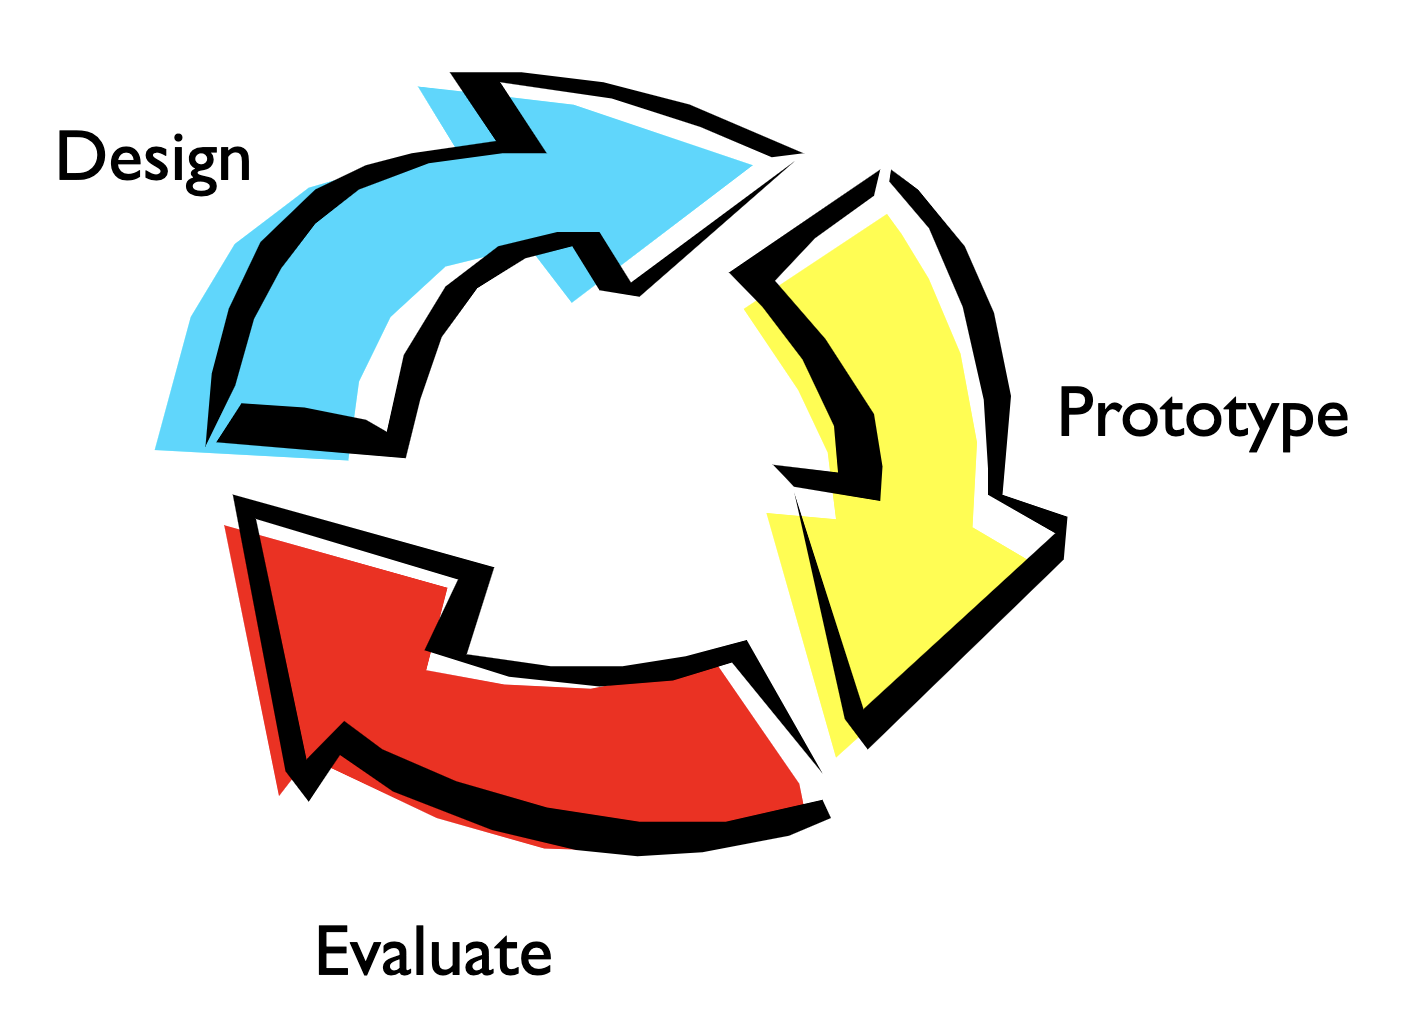
\includegraphics[scale=0.15]{lectures/wk1/img/cycle.png}
\end{center}

\subsection{Contextual Inquiry}
Observe existing practices.

Create scenarios of actual use.

Create models to gain insight  into work processes.

\subsection{Rapid Prototyping}
Low fidelity can be better as it is:
\begin{itemize}
    \item Fast, no attachment if you have to scrap it (if you were invested in it then you will stick with a bad UI due to the sunk-cost fallacy).
    \item No need to debug
\end{itemize}

\subsection{Evaluation}
\textbf{Test with real target users.}

Ask other CS 160 UI experts to check a UI for potential accessibility problems using the heuristics and conditions they learned to look for.


\subsection{Goals of the Course}
Learn to design, prototype, evaluate interfaces:
\begin{itemize}
    \item Discover tasks of prospective users
    \item Cognitive/perceptual constraints that effect design
    \item Techniques for evaluating an interface design
    \item Importance of iterative design for usability
    \item Technology used to prototype \& implement UI code
    \item Unique aspects of intelligent user interfaces
    \item How to work together on a team project
    \item Communicate your results to a group
\end{itemize}
These will likely be very important for future jobs.

$\hrulefill$

In other CS classes, you learn algorithms. Here we expect you to know algorithms and teach design.

\subsection{Teams}
\textbf{Instructors will form groups of 4-5 students (who are in the same section) in week 2 or 3.}

\subsection{Course Mechanics}
You must be comfortable with programming at the level of CS61B. 

Note: Individual programming assignments require you to write code in Javascript, HTML, CSS.

You must be able to attend class and one of the sections each week.

You must commit to working with your assigned team on your group project.

\subsection{Office Hours}
TBD

\subsection{Sections}
4 options: 
\begin{enumerate}
    \item 101 – Wed 11am-12pm, 540 Cory
    \item 102 - Fri 1-2pm, 310 Soda
    \item 103 – Th 10am-11am, 540 Cory
    \item 104 – Wed 2 -3pm, 320 Soda
\end{enumerate}
You MUST be able to attend one of the sections.

\textbf{Section starts next week}

1st half of the semester: Lecture material + Tech stack 
2nd half of the semester: Design critiques

\subsection{Readings}
Readings will be posted on bCourses.

Reading responses (recurring assignment)
You must post a substantial answer for each assigned reading, \textbf{by 10am before class} (so we can review them before class). 

Responses are the major factor in your \textit{class participation grade}.

\textbf{Your first reading response is due next Tuesday by 10am.}

\subsection{Grading}
\begin{enumerate}
    \item Participation – 10\% (Reading responses, class, Ed Discussions)
    \item Individual Assignments 20\%
    \item Two Midterms 30\%
    \item Group Project Assignments 40\%
\end{enumerate}
Note that we generally do the midterms in-class and this may not be accurate -- check bCourses.

\subsubsection{Late Assignments}
\begin{itemize}
    \item Most assignments will be due before class on the due date
    \item Individual assignments lose 20\% per day (weekend counts as one day)
    \item Group assignments will not be accepted late
\end{itemize}
